 \chapter{Interviewing the Data}
\emph{We begin our analysis with descriptive findings from our dataset.
These findings describe the basic behavior and nature of how Twitter users share the news online.}

\section{The Big Picture}
% This left a total of 2,658 distinct articles (38%) shared in 123,113 (89%) tweets by 20,956 Twitter users (93%).
 

Of the 2,658 articles shared 123,133 times on Twitter that we track in our studies, the vast majority are shared less than 100 times. Story sharing behavior follows an approximate power law distribution.  

\begin{figure}[H]  
\centering 
  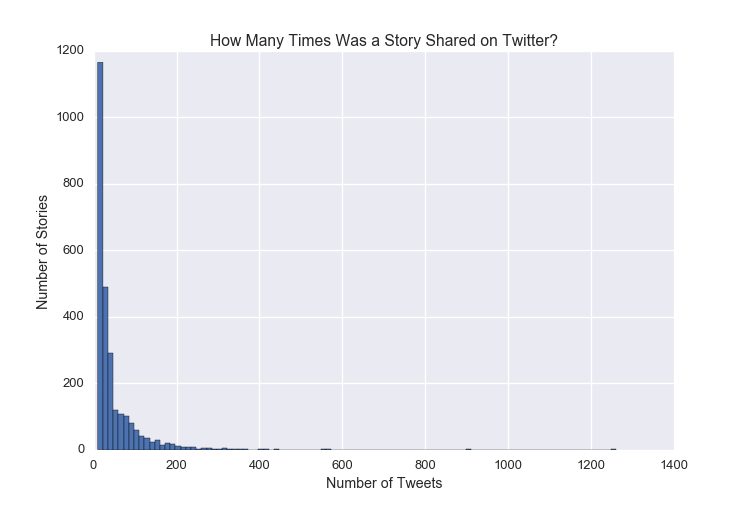
\includegraphics[width=0.8\textwidth]{story-share-dist}  
  \caption{Distribution of Story Shares
    \label{fig:story-share-dist}}
\end{figure} 

On average, stories are shared 46 times, however, the median (50th percentile) of shares is just 26. 

%%%
CNN politico and fox lead the most popular publications to be tweeted about... likely due to the political nature of the outlets.

\begin{figure}[H]  
\centering 
  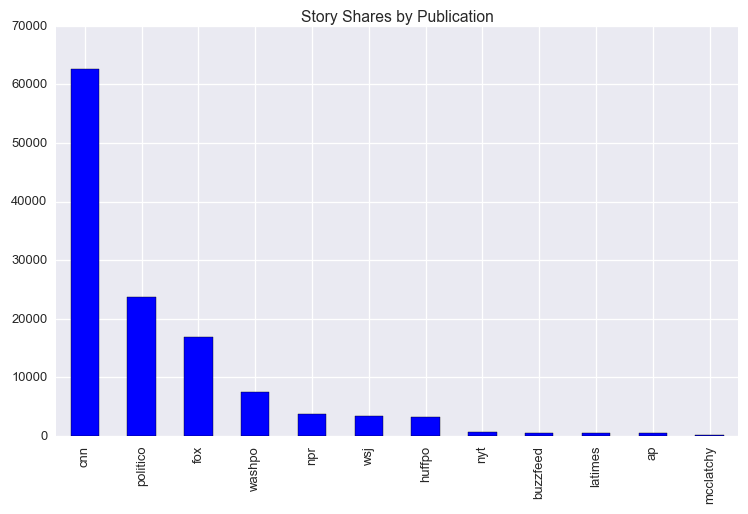
\includegraphics[width=0.8\textwidth]{all-stories-by-pub}  
  \caption{Number of story shares by publication
    \label{fig:tweets-by-pub}}
\end{figure} 
 


\newpage

CNN & Politico also lead the top 10 most popular stories.
Trump is by far the most tweetable candidate
 
\begin{table}
%\begin{tabular}{| l || c |} 
\begin{tabular}{ |l c| } 
    %s\toprule
    \hline
    Article &  \# tweets \\
    \hline
    %\midrule
    The One Weird Trait That Predicts Whether You're a Trump Supporter &   1260 \\
    Donald Trump Is Shocking, Vulgar and Right                         &    901 \\
    Biden praises Sanders on income inequality                         &    563 \\
    Why I'm voting for Trump                                           &    554 \\
    Anne Frank's stepsister compares Donald Trump to Adolf Hitler      &    445 \\
    Trump basks in his spotlight                                       &    436 \\
    Rubio: Law-abiding undocumented immigrants could stay              &    413 \\
    Terrorists use Trump's `Muslim ban' speech in recruitment video    &    398 \\
    Iowa caucuses: Donald Trump's moment of truth                      &    364 \\
    GOP senators: If Cruz wins, we lose                                &    357 \\
    %\bottomrule
    \hline
\end{tabular}
\caption{\label{tab:top-10}Top 10 Shared Stories}
\end{table}



%% Same table but include Publication

% \begin{table}
% %\begin{tabular}{| l || c |} 
% \begin{tabular}{ |l c c| } 
%     \hline
                                                            
%     Article & Publication &   \# tweets    \\
%     GOP senators: If Cruz wins, we lose & cnn &   357 \\
%     Iowa caucuses: Donald Trump's moment of truth &  cnn   &   364 \\
%     Terrorists use Trump's `Muslim ban' speech in recruitment video &   cnn  &   398 \\
%     Rubio: Law-abiding undocumented immigrants could stay & politico &   413 \\
%     Trump basks in his spotlight & cnn &   436 \\
%     Anne Frank's stepsister compares Donald Trump to Adolf Hitler &  cnn   &   445 \\
%     Why I'm voting for Trump &  cnn   &   554 \\
%     Biden praises Sanders on income inequality &   cnn  &   563 \\
%     Donald Trump Is Shocking, Vulgar and Right & politico &   901 \\
%     The One Weird Trait That Predicts Whether You’re a Trump Supporter &  cnn   &  1260 \\
%     \hline
% \end{tabular}
% \caption{\label{tab:top-10}Top 10 Shared Stories}
% \end{table}


 















  
 


% \section{Tweets}

% \begin{figure}[H]  
% \centering 
%   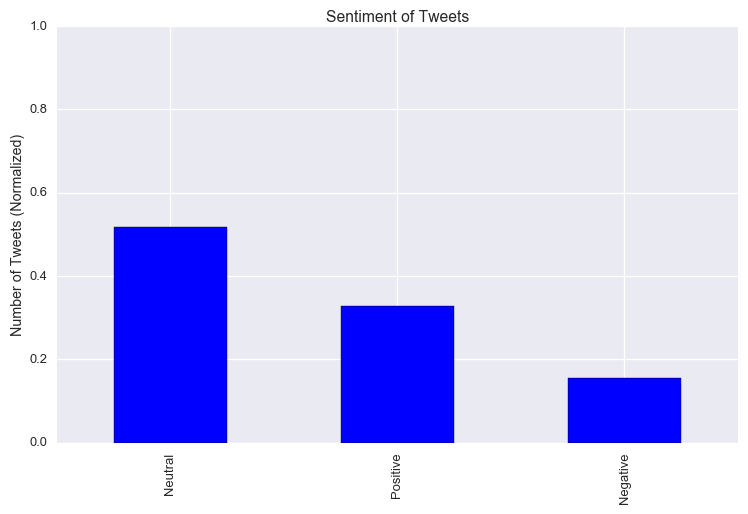
\includegraphics[width=0.9\textwidth]{all-tweets-sentiment}  
%   \caption{Sentiment of Tweets
%     \label{fig:data-stack-Twitter}}
% \end{figure} 


% \section{Tweeters}


%  \subsection{Descriptives}
%  \subsection{Story Length}
%  \subsection{Emotionality}
%  \subsection{Positivity}

%   \section{By Candidate}
%  \subsection{Descriptives}
%  \subsection{Story Length}
%  \subsection{Emotionality}
%  \subsection{Positivity}


%   \section{By Degree of Political Engagement}
%  \subsection{Descriptives}
%  \subsection{Story Length}
%  \subsection{Emotionality}
%  \subsection{Positivity}

%  \section{Trust and Virality? Test}